We introduce the following notation: we denote directed and labeled multi-graphs as $G = (\mathcal{V}, \mathcal{E}, \mathcal{R})$ with nodes (entities) $v_i \in \mathcal{V}$ and labeled edges (relations) $(v_i, r, v_j) \in \mathcal{E}$, where $r\in\mathcal{R}$ is a relation type.\footnote{$\mathcal{R}$ contains relations both in canonical direction (e.g. \textit{born\_in}) and in inverse direction (e.g. \textit{born\_in\_inv}).}

\subsection{Relational graph convolutional networks}
Our model is primarily motivated as an extension of GCNs that operate on local graph neighborhoods \cite{duvenaud2015convolutional,kipf2016semi} to large-scale relational data. These and related methods such as graph neural networks \cite{scarselli2009graph} can be understood as special cases of a simple differentiable message-passing framework \cite{gilmer2017neural}:
\begin{equation}
\label{eq:message-passing}
h_i^{(l+1)}= \sigma \left( \sum_{m \in \mathcal{M}_i} g_m(h_i^{(l)}, h_j^{(l)}) \right),
\end{equation}
where $h_i^{(l)}\in\mathbb{R}^{d^{(l)}}$ is the hidden state of node $v_i$ in the $l$-th layer of the neural network, with $d^{(l)}$ being the dimensionality of this layer's representations. Incoming messages of the form $g_m(\cdot, \cdot)$ are accumulated and passed through an element-wise activation function $\sigma(\cdot)$, such as the $\mathrm{ReLU}(\cdot)=\max(0,\cdot)$.\footnote{Note that this represents a simplification of the message passing neural network proposed in \cite{gilmer2017neural} that suffices to include the aforementioned models as special cases.} $\mathcal{M}_i$ denotes the set of incoming messages for node $v_i$ and is often chosen to be identical to the set of incoming edges. $g_m(\cdot, \cdot)$ is typically chosen to be a (message-specific) neural network-like function or simply a linear transformation $g_m(h_i, h_j)=W h_j$ with a weight matrix $W$ such as in \citet{kipf2016semi}.

This type of transformation has been shown to be very effective at accumulating and encoding features from local, structured neighborhoods, and has led to significant improvements in areas such as graph classification \cite{duvenaud2015convolutional} and graph-based semi-supervised learning \cite{kipf2016semi}.

Motivated by these architectures, we define the following simple propagation model for calculating the forward-pass update of an entity or node denoted by $v_i$ in a relational (directed and labeled) multi-graph:
\begin{equation}
\label{eq:layer}
h_i^{(l+1)}= \sigma \left( \sum_{r \in \mathcal{R}}\sum_{j \in \mathcal{N}^r_i} \frac{1}{c_{i,r}}W_r^{(l)} h_j^{(l)} + W_0^{(l)}h_i^{(l)} \right),
\end{equation}
where $\mathcal{N}^r_i$ denotes the set of neighbor indices of node $i$ under relation $r\in\mathcal{R}$. $c_{i,r}$ is a problem-specific normalization constant that can either be learned or chosen in advance (such as $c_{i,r}=|\mathcal{N}^r_i|$).

Intuitively, (\ref{eq:layer}) accumulates transformed feature vectors of neighboring nodes through a normalized sum. Different from regular GCNs, we introduce relation-specific transformations, i.e. depending on the type and direction of an edge.
To ensure that the representation of a node at layer $l+1$ can also be informed by the corresponding representation at layer $l$, we add a single self-connection of a special relation type to each node in the data. Note that instead of simple linear message transformations, one could choose more flexible functions such as multi-layer neural networks (at the expense of computational efficiency). We leave this for future work.

A neural network layer update consists of evaluating (\ref{eq:layer}) in parallel for every node in the graph. In practice, (\ref{eq:layer}) can be implemented efficiently using sparse matrix multiplications to avoid explicit summation over neighborhoods. Multiple layers can be stacked to allow for dependencies across several relational steps. We refer to this graph encoder model as a relational graph convolutional network (R-GCN). The computation graph for a single node update in the R-GCN model is depicted in Figure \ref{fig:model}.

\begin{figure}[t!]
        \centering
    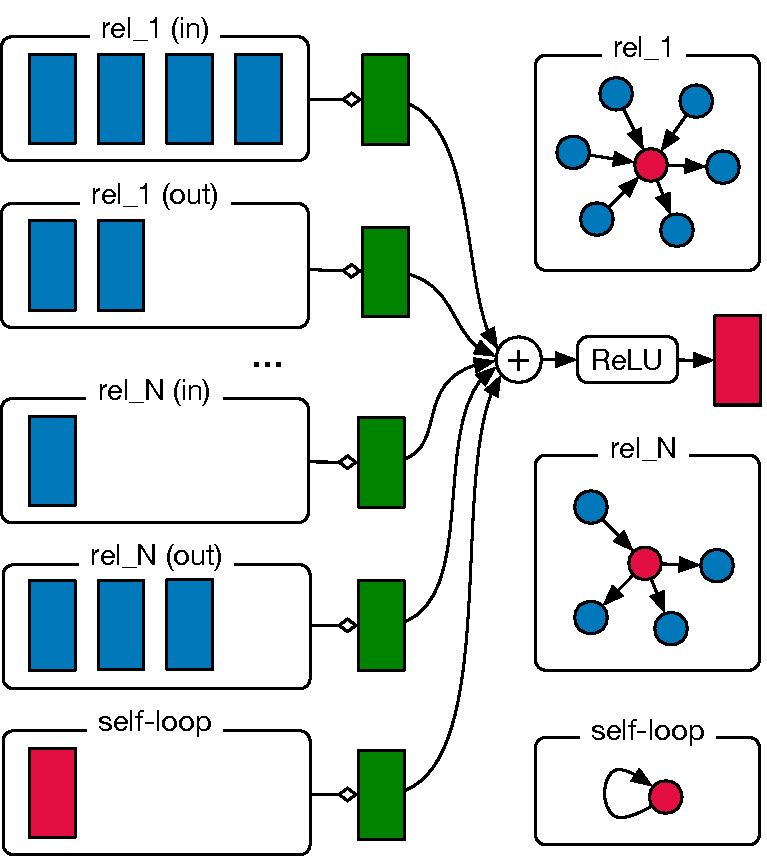
\includegraphics[width=0.8\linewidth]{figures/rgcn-layer.pdf}
    \label{fig:model-a}
    \caption{Diagram for computing the update of a single graph node/entity (red) in the R-GCN model. Activations ($d$-dimensional  vectors) from neighboring nodes (dark blue) are gathered and then transformed for each relation type individually (for both in- and outgoing edges). The resulting representation (green) is accumulated in a (normalized) sum and passed through an activation function (such as the ReLU). This per-node update can be computed in parallel with shared parameters across the whole graph.}
    \label{fig:model}
\end{figure}

\subsection{Regularization}
A central issue with applying (\ref{eq:layer}) to highly multi-relational data is the rapid growth in number of parameters with the number of relations in the graph. In practice this can easily lead to overfitting on rare relations and to models of very large size.

To address this issue, we introduce two separate methods for regularizing the weights of R-GCN-layers: \textit{basis}- and \textit{block-diagonal}-decomposition. With the basis decomposition, each $W_r^{(l)}$ is defined as follows:
\begin{equation}
\label{eq:basis}
W_r^{(l)} = \sum_{b=1}^B a_{rb}^{(l)} V_b^{(l)},
\end{equation}
i.e.~as a linear combination of basis transformations $V_b^{(l)}\in\mathbb{R}^{d^{(l+1)}\times d^{(l)}}$ with coefficients $a_{rb}^{(l)}$ such that only the coefficients depend on \textit{r}. In the block-diagonal decomposition, we let each $W_r^{(l)}$ be defined through the direct sum over a set of low-dimensional matrices:
\begin{equation}
\label{eq:block}
W_r^{(l)} = \bigoplus_{b=1}^B Q^{(l)}_{br}.
\end{equation}
Thereby, $W_r^{(l)}$ are block-diagonal matrices:
$\mathrm{diag}(Q^{(l)}_{1r}, \ldots, Q^{(l)}_{Br})$ with $Q^{(l)}_{br} \in \mathbb{R}^{(d^{(l+1)}/B)\times( d^{(l)}/B)}$.

The basis function decomposition \eqref{eq:basis} can be seen as a form of effective weight sharing between different relation types, while the block decomposition \eqref{eq:block} can be seen as a sparsity constraint on the weight matrices for each relation type. The block decomposition structure encodes an intuition that latent features can be grouped into sets of variables which are more tightly coupled within groups than across groups.
Both decompositions reduce the number of parameters needed to learn for highly multi-relational data (such as realistic knowledge bases). At the same time, we expect that the basis parameterization can alleviate overfitting on rare relations, as parameter updates are shared between both rare and more frequent relations.

The overall R-GCN model then takes the following form: We stack $L$ layers as defined in \eqref{eq:layer} -- the output of the previous layer being the input to the next layer. The input to the first layer can be chosen as a unique one-hot vector for each node in the graph if no other features are present. For the block representation, we map this one-hot vector to a dense representation through a single linear transformation. While we only consider such a featureless approach in this work, we note that it was shown in \citet{kipf2016semi} that it is possible for this class of models to make use of pre-defined feature vectors (e.g.~a bag-of-words description of a document associated with a specific node).
